\documentclass[acmtog]{acmart}
\usepackage{graphicx}
\usepackage{subfigure}
\usepackage{natbib}
\usepackage{listings}
\usepackage{bm}
\usepackage{amsmath}

\definecolor{blve}{rgb}{0.3372549 , 0.61176471, 0.83921569}
\definecolor{gr33n}{rgb}{0.29019608, 0.7372549, 0.64705882}
\makeatletter
\lst@InstallKeywords k{class}{classstyle}\slshape{classstyle}{}ld
\makeatother
\lstset{language=C++,
	breaklines=true,
	basicstyle=\ttfamily,
	keywordstyle=\color{blve}\ttfamily,
	stringstyle=\color{red}\ttfamily,
	commentstyle=\color{magenta}\ttfamily,
	morecomment=[l][\color{magenta}]{\#},
	classstyle = \bfseries\color{gr33n},
	tabsize=2,
	morekeywords={Vec3f, Interaction},
}
\lstset{basicstyle=\ttfamily}



% Title portion
\title{Assignment 5: {Cloth Animation}}

\author{Name:\quad Bingnan Li \\ student number:\ 2020533092
\\email:\quad libn@shanghaitech.edu.cn}

% Document starts
\begin{document}
\maketitle

\vspace*{2 ex}

\section{Introduction}
\begin{itemize}
	\item Force computation with Hooke's law.
	\item Structural, shear, and bending springs.
	\item Fix the location of two mesh points to stop the cloth falling down.
	\item Real-time and stable animation.
	\item Apply external forces to the cloth to simulate the behavior of wind.
	\item Add a sphere or cube obstacle to simulate a piece of cloth falling on a sphere or a cube with collision handling.
	\item Drag a mesh point to move the cloth with mouse in real-time.
\end{itemize}

\section{Implementation Details}
\begin{enumerate}
	\setlength{\parindent}{2em}
	\item Force computation with Hooke's law.
	\par By Hooke's law, we have 
	\[f = k \Delta x\]
	where $k$ is stiffness.
	\par Hence, the programming code is 
	\begin{lstlisting}
Vec3 ComputeHookeForce(int iw_this, int ih_this, int iw_that, int ih_that, Float dx_world) const {

size_t this_idx, that_idx;

if (!Get1DIndex(iw_this, ih_this, this_idx) || !Get1DIndex(iw_that, ih_that, that_idx)) {
return {0, 0, 0};
}

Vec3 p = local_or_world_positions.at(this_idx);
Vec3 q = local_or_world_positions.at(that_idx);
Vec3 dis = p - q;

return stiffness * (dx_world - glm::length(dis)) * glm::normalize(dis);
}		
	\end{lstlisting}
	\item Structural, shear, and bending springs.
	\par By this illustration,
	\begin{figure}[H]
	\centering
	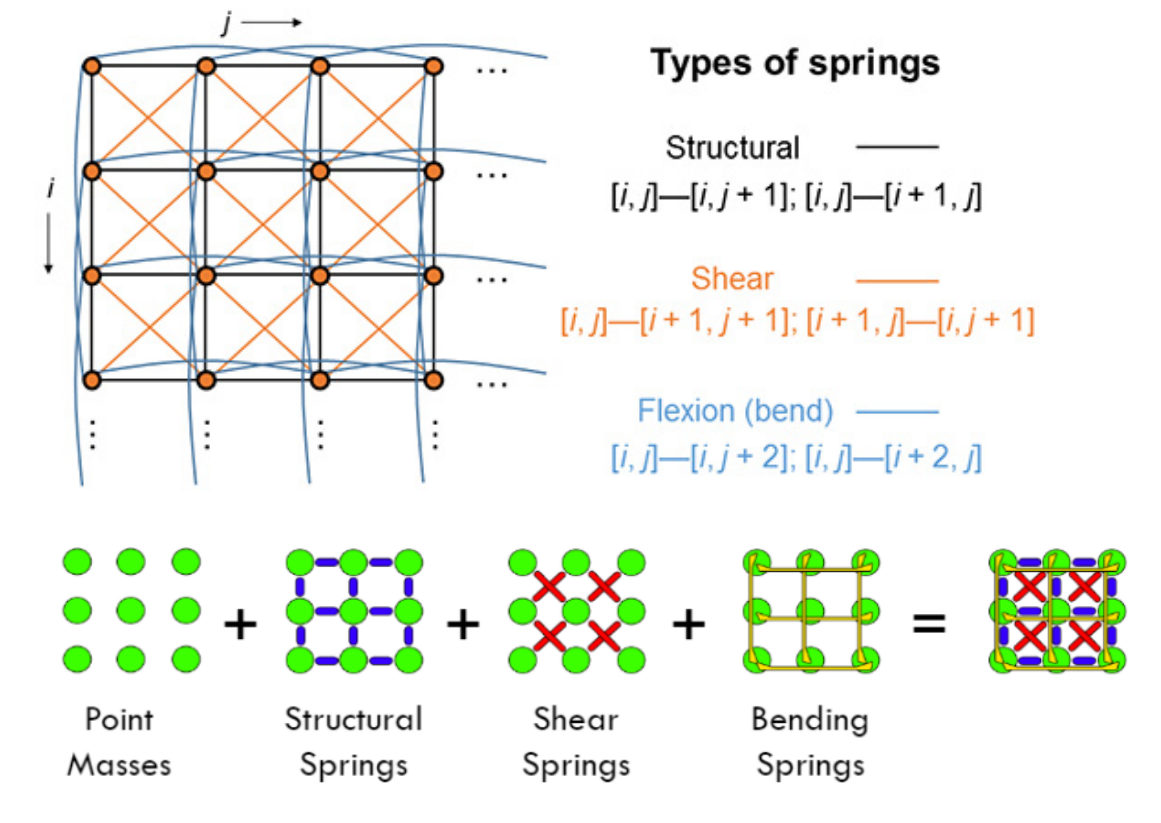
\includegraphics[width=0.45\textwidth]{images/hook_force.png}
	\caption{simple box}
	\end{figure}
	\par we know that the spring force contains three types of forces, which are structural, shear and bending forces. Thus, we have the following code
	\begin{lstlisting}
Vec3 RectCloth::ComputeSpringForce(int iw, int ih) const {

	const Vec3 scale = object->transform->scale;

	Vec3 springForce(0);
	size_t idx;
	if (!Get1DIndex(iw, ih, idx) || is_fixed_masses.at(idx)) {
		return springForce;
	}

	springForce += ComputeHookeForce(iw, ih, iw, ih - 1, dx_local);
	springForce += ComputeHookeForce(iw, ih, iw, ih + 1, dx_local);
	springForce += ComputeHookeForce(iw, ih, iw - 1, ih, dx_local);
	springForce += ComputeHookeForce(iw, ih, iw + 1, ih, dx_local);

	springForce += ComputeHookeForce(iw, ih, iw - 1, ih - 1, (float) std::sqrt(2) * dx_local);
	springForce += ComputeHookeForce(iw, ih, iw - 1, ih + 1, (float) std::sqrt(2) * dx_local);
	springForce += ComputeHookeForce(iw, ih, iw + 1, ih - 1, (float) std::sqrt(2) * dx_local);
	springForce += ComputeHookeForce(iw, ih, iw + 1, ih + 1, (float) std::sqrt(2) * dx_local);

	springForce += ComputeHookeForce(iw, ih, iw, ih - 2, 2 * dx_local);
	springForce += ComputeHookeForce(iw, ih, iw, ih + 2, 2 * dx_local);
	springForce += ComputeHookeForce(iw, ih, iw - 2, ih, 2 * dx_local);
	springForce += ComputeHookeForce(iw, ih, iw + 2, ih, 2 * dx_local);

	return springForce;
}
	\end{lstlisting}
	\item Damping.
	\par Once we get new spring force and gravity, we need to add damping so that the cloth would not keep fluctuating.
	\par By the physical inference, we have
	\[a = TotalForce - damping\_ration\times v \] 
	Thus, we have the following code:
	\begin{lstlisting}
void RectCloth::ComputeAccelerations() {
	std::normal_distribution<float> nd(ud(gen), 2 * std::max(ud(gen), 5.0f));
	for (int w = 0; w < mass_dim.x; ++w) {
		for (int h = 0; h < mass_dim.y; ++h) {
			size_t idx;
			if (Get1DIndex(w, h, idx) && !is_fixed_masses.at(idx)) {
				world_accelerations.at(idx) =
						(ComputeSpringForce(w, h) - damping_ratio * world_velocities.at(idx)) / mass_weight;
			}
		}
	}
}
	\end{lstlisting}
	\item External force
	\par In order to add external force, we need to add a new random acceleration to the total acceleration.
	\item Collision with sphere.
	\par Once a mass was fell into the sphere, we firstly set its position to the surface of sphere along the normal direction. Then, we need to set the component along the normal direction of velocity to zero. Therefore, we have the following code:
	\begin{lstlisting}
if (glm::distance(local_or_world_positions.at(i), SphereCenter) < R) {
	Vec3 normal = glm::normalize(local_or_world_positions.at(i) - SphereCenter);
	local_or_world_positions.at(i) = SphereCenter + R * normal;
	Vec3 v_n_component = glm::dot(world_velocities.at(i), normal) * normal;
	world_velocities.at(i) -= v_n_component;
}
	\end{lstlisting}
	\item Interactive points
	\par In order to achieve interaction, we first generate a ray based on the mouse position. We can use $glm::unproject$ function to do that. After that, we need to check all masses about whether the ray interacts with a sphere whose sphere center is the location of mass and a radius 0.05. If it did, then we set its velocity to zero and a drag index to its index.
	\par After that, once the drag index in not -1, we set the dragged point to the new position based on the new mouse position.
	\par Hence, we have the following code:
	\begin{lstlisting}
if (drag_idx != -1 && Input::GetMouseButton(0)) {
	Vec3 p = local_or_world_positions.at(drag_idx);
	world_velocities.at(drag_idx) = Vec3(0);
	local_or_world_positions.at(drag_idx) = GetDragPos(p);
	return;
}

if (Input::GetMouseButton(0)) {
	Vec3 dir = glm::normalize(GetWorldPosFromCursor() - cam->transform.position);
	for (size_t i = 0; i < length; ++i) {
		if (Interact(cam->transform.position, dir, i)) {
			world_velocities.at(i) = Vec3(0);
			drag_idx = (int) i;
			break;
		}
	}
} else {
	drag_idx = -1;
}
	\end{lstlisting} 
	
\end{enumerate}
\section{Results}
pictures should be in
\begin{figure}[H]
	\centering
	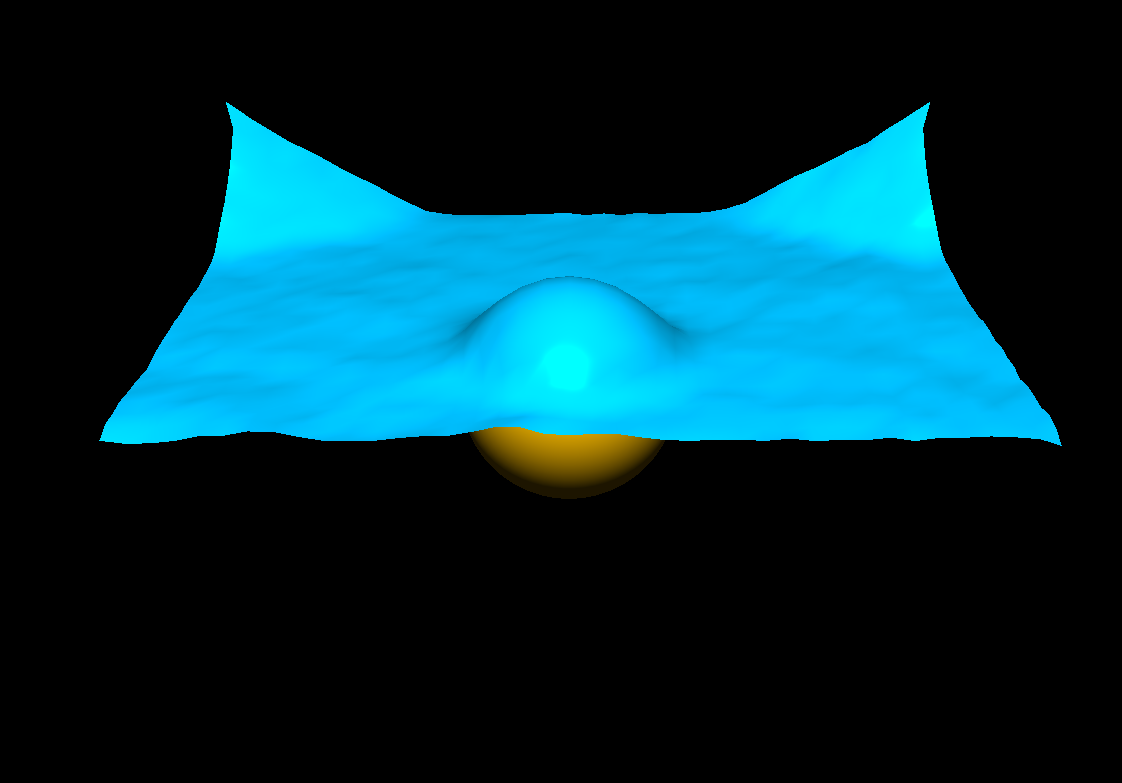
\includegraphics[width=0.45\textwidth]{images/1.png}
	\caption{Sphere Collision}
\end{figure}
\begin{figure}[H]
	\centering
	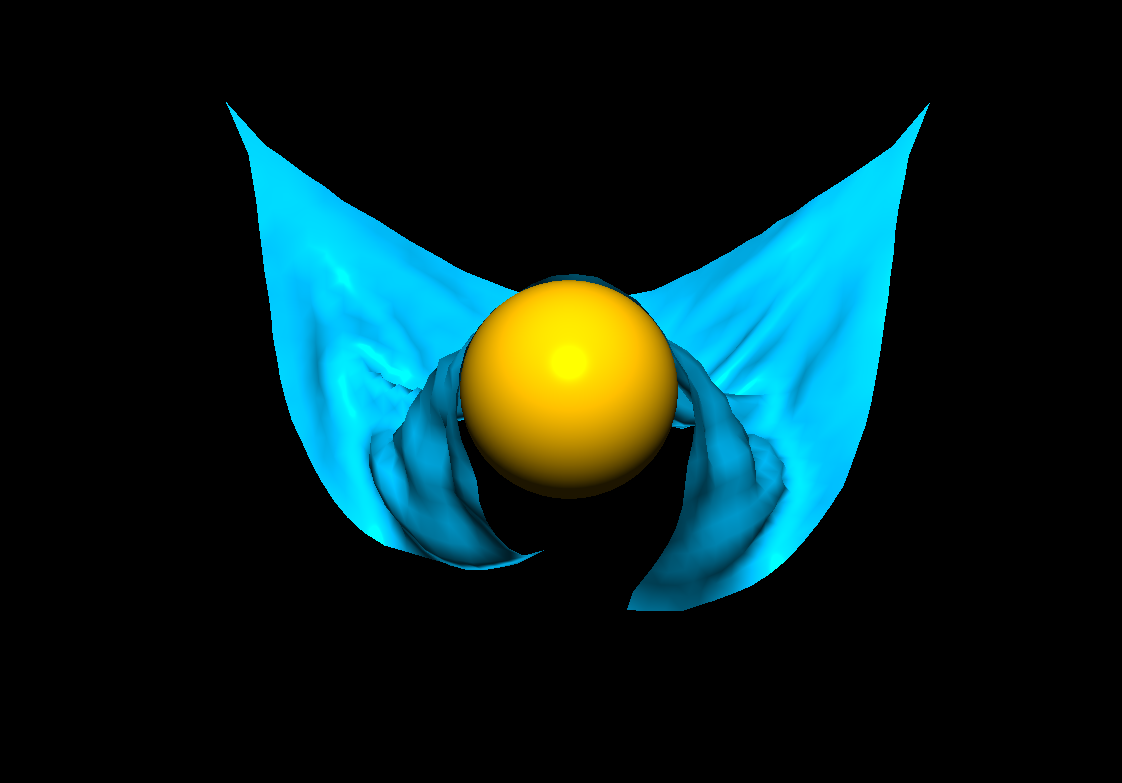
\includegraphics[width=0.45\textwidth]{images/2.png}
	\caption{Sphere Collision}
\end{figure}
\begin{figure}[H]
	\centering
	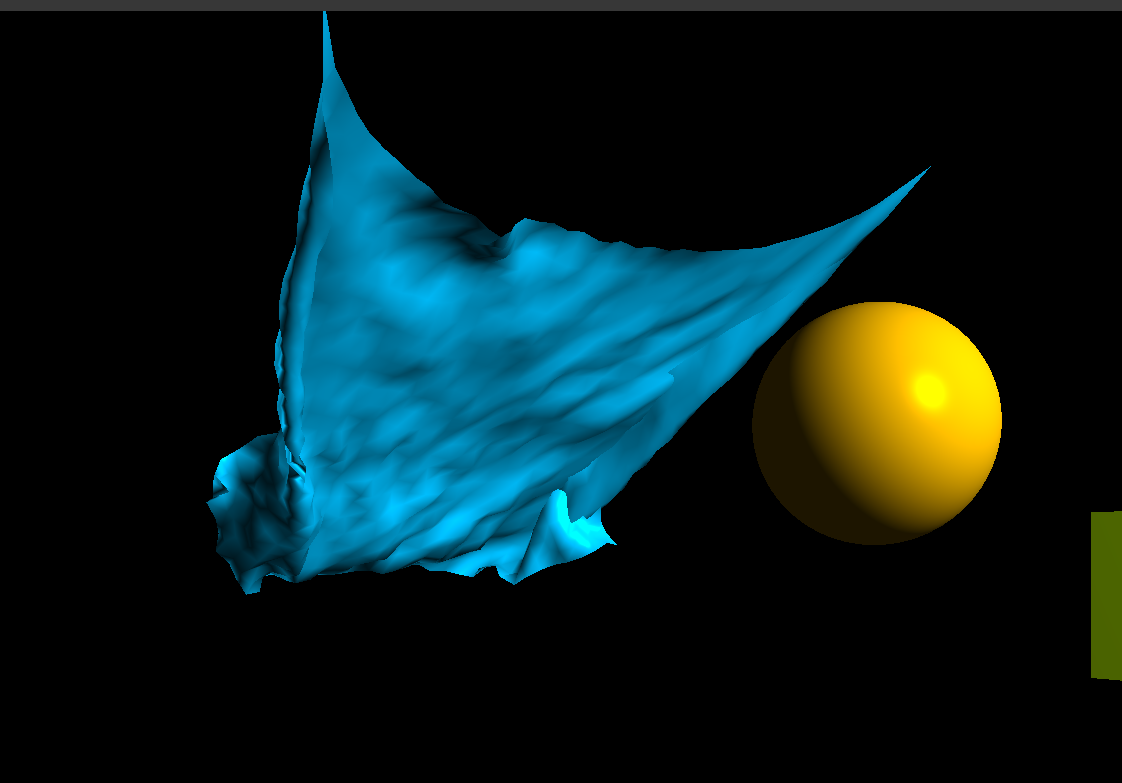
\includegraphics[width=0.45\textwidth]{images/3.png}
	\caption{Sphere Collision}
\end{figure}


\begin{figure}[H]
	\centering
	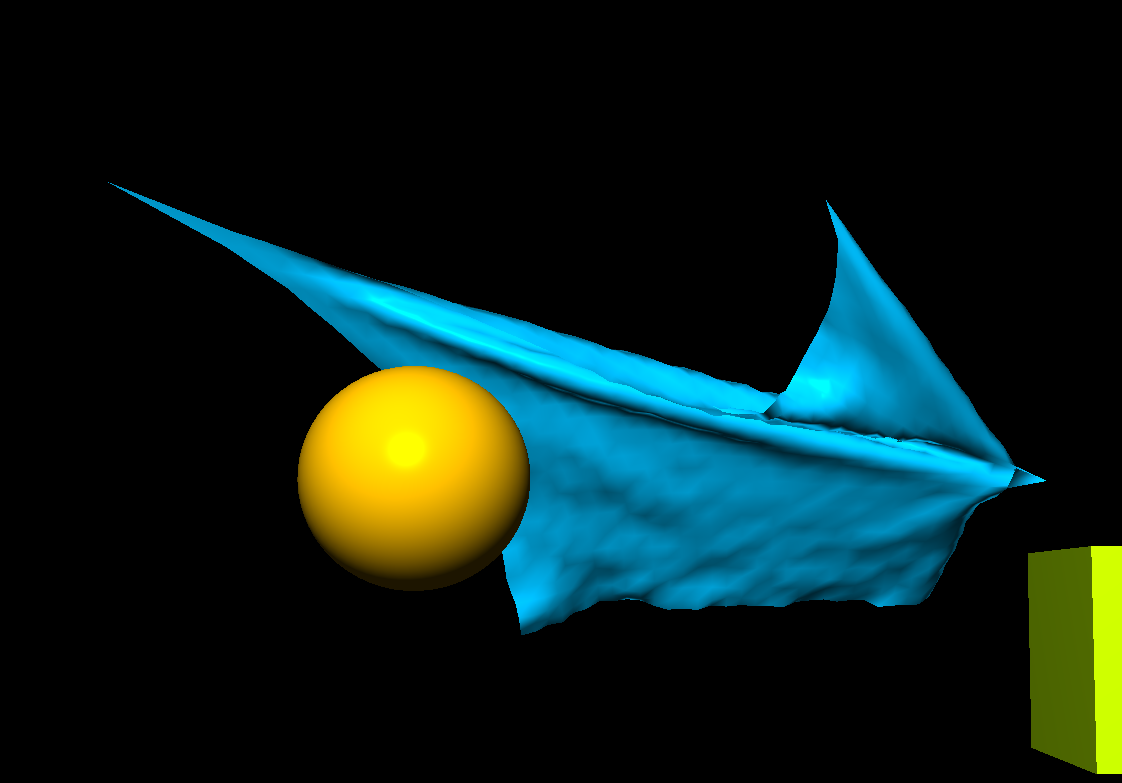
\includegraphics[width=0.45\textwidth]{images/4.png}
	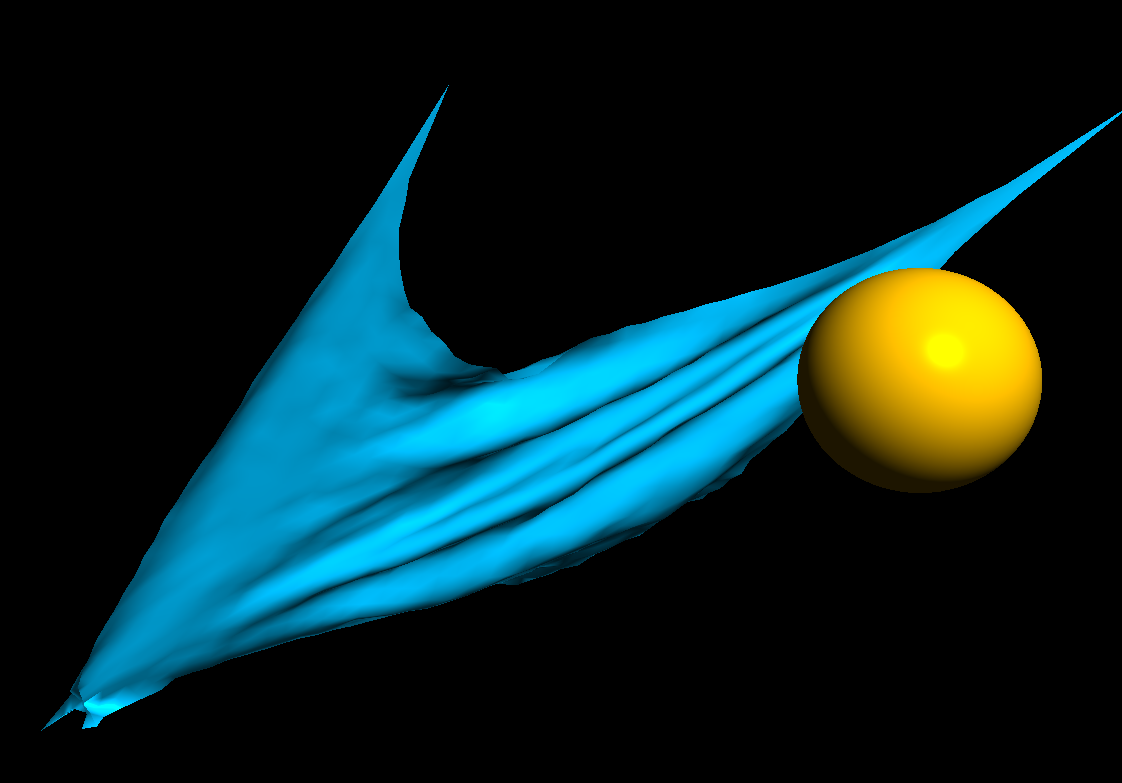
\includegraphics[width=0.45\textwidth]{images/5.png}
	\caption{Interactive points}
\end{figure}

\end{document}
